\documentclass[aspectratio=169]{beamer}
\usetheme{Berlin}
\usecolortheme{beaver}


\usepackage[utf8]{inputenc}
%\usepackage[T1]{fontenc}
%\usepackage{lmodern}
\usepackage{amsmath,amssymb,amsthm,mathrsfs,amsfonts, amstext}  
\usepackage{mathtools}
\usepackage{listings}
\usepackage[english]{babel}
\usepackage{verbatim}
\usepackage{pgfplots}
%\usepackage{amssymb, amsmath, amsbsy} % simbolitos
%\usepackage{upgreek} % para poner letras griegas sin cursiva
%\usepackage{cancel} % para tachar
%\usepackage{mathdots} % para el comando \iddots
%\usepackage{mathrsfs} % para formato de letra
%\usepackage{stackrel} % para el comando \stackbin
\usepackage{graphicx}
\usepackage{grffile}
\graphicspath{ {../images/} }
\usepackage{caption}
\usepackage{chngcntr}
\usepackage{etoolbox} % needed for the code below
\usepackage{hyperref}
\usepackage{multimedia}
\usepackage{algpseudocode}
\usepackage{tikz}
\usepackage{IEEEtrantools}
\usepackage{physics}
\usepackage{pgfpages}
\usepackage{booktabs}
\usepackage{amsfonts}
\usepackage{siunitx}

\captionsetup[figure]{labelformat=empty}% redefines the caption setup of the figures environment in the beamer class.

%\setbeameroption{show only notes}
%\setbeameroption{show notes on second screen=right}
\DeclareMathOperator{\Ra}{Ra}
\newcommand{\jump}[1]{\ensuremath{[\![ #1 ]\!]}}
\newcommand{\avg}[1]{\ensuremath{\{\mspace{-6mu}\{#1\}\mspace{-6mu}\}}}

\let\oldfootnotesize\footnotesize
\renewcommand*{\footnotesize}{\oldfootnotesize\tiny}

\AtBeginSection[]
{
	\begin{frame}
	\frametitle{Overview}
	\tableofcontents[currentsection]
	\end{frame}
}

\setbeamercolor{block title}{use=structure,fg=white,bg=red!75!black}
\setbeamercolor{block body}{use=structure,fg=black,bg=red!5!white}
\setbeamertemplate{itemize item}{\color{red!90!black}$\blacktriangleright$}
\setbeamertemplate{itemize subitem}{\color{red!50!black}$\blacktriangleright$}
\setbeamercolor{section number projected}{fg=white,bg=red!60!black}
\setbeamercolor{subsection number projected}{parent=section number projected}


\bibliographystyle{alpha}


%%%%%%% math definitions %%%%%%%%%%


%%%%%%%%%%%%%%%%%%%%%%%%%%%%%%%%%%%%%%%%%%%%%%


%%%%%%%%%%%%%%%%%%%%%%%%%%%%%%%%%%%

\title{Competitive Hebbian learning through spike-timing-dependent synaptic plasticity - A summary \cite{article}}
\author{Jonas Wildberger}
\begin{document}

\begin{frame}
  \titlepage
\end{frame}

\begin{frame}{Overview}
  \tableofcontents
\end{frame}

\section{Motivation}
\begin{frame}{Motivation}

		Hebbian learning:
			\begin{itemize}
				\item Synapse connecting neurons that are repeatedly active at the same time becomes stronger
				\item Different synapses compete with each other: The strengthening of one leads to the weakening of another
			\end{itemize}

	\begin{center}
	\visible<2->{What are biophysically realistic explanations for this behaviour?}
	\end{center}
	\visible<3->{Song et. al: Spike-timing dependent plasticity (STDP) naturally leads to a stationary distribution of synaptic conductances that enables competition among synapses}
\note{AIMD: First principles, quantum mechanics, DFT. Computational costs: 100 ps, 100s of atoms, empirica FF: based on approximations and experimental data}
\note{Data: Atomic configurations and corresponding potential energies, learn this functional dependence}
\note{real system invariant to permutations, translations, rotations, so model needs too. Auxiliary quantities: Symmetry functions (describe local geometric environment, problem: ad hoc), coulomb matrix entries: distinct inverse distances between all atoms, problem: extened periodic systems}
\end{frame}
\note{Convection: transfer of heat by the movement of the fluid\\
	Natural: motion generated by density differences, not by external sources\\
Applications: Nuclear reactor design,
cooling of electronic eqiupment,
heating and ventialtion in the design
of buildings\\
Goal: Identify different flow patterns and investigate which method is suited better}

\section{The model}
\begin{frame}{STDP}
	\begin{columns}
		\begin{column}{0.5\textwidth}
 Function describing change in synaptic conductances
				$$F(\Delta t ) = \begin{cases}
				A_+ \exp(\Delta t/\tau_+), & \text{if } \Delta t < 0 \\
				- A_- \exp(-\Delta t/\tau_-), & \text{if } \Delta t \geq 0
				\end{cases}$$
				Presynaptic spikes / Postsynaptic action potential: Strengthening\\
				Postsynaptic action potential / Presynaptic spikes: Weakening

		\end{column}
		\begin{column}{0.5\textwidth}
			\begin{figure}
				
				\centering
				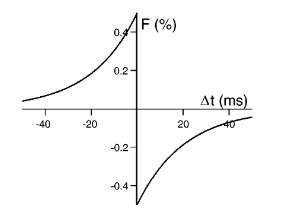
\includegraphics[width=0.8\textwidth]{CN1}
				\caption{Dependence of synaptic conductances on $\Delta t$ \cite{article}}
			\end{figure}
		\end{column}
	\end{columns}
\note{$\tau_+ = \tau_-\approx 20$ms: ranges in which pre- and postsynaptic adaptation occurs\\
	$A_-, A_+$: maximum amount of modification when $\Delta t \rightarrow 0$; $A_- /A_+ = 1.05$}
\note{Figure: Water, e x O-H bond, e z perpendicular to plane of water molecule }
\note{other option for D i j angular information as well x ij cartesian coordinates of R i j}
\end{frame}
\begin{frame}{The simulation}

\begin{itemize}
	\item<1-> Integrate-and-fire model neuron with 1000 excitatory synapses and 200 inhibitory synapses
	\item<2-> Inhibitory synapses are kept fixed with input frequency of 10 Hz.
	\item<3-> Excitatory synapses initialised with maximum values $g_{\max}$; adapted according to STDP with input frequencies of 10Hz and 40Hz
\end{itemize}

\note{NN: fixed input size, append 0s potentially}
\end{frame}
\begin{frame}{Stationary distribution I}

\begin{columns}
	\begin{column}{0.5\textwidth}
	\begin{itemize}
		\item<1-> At the beginning: Mean input already brings the neuron's potential above its activation threshold\\
		$\Rightarrow$ synapses are weakened according to $F$
		\item<2-> Eventually excitatory inputs balance inhibitory effects: \textcolor{darkred}{Stationary distribution}
		
	\end{itemize}
		
	\end{column}
	\begin{column}{0.5\textwidth}
		\begin{figure}
			
			\centering
			\visible<3>{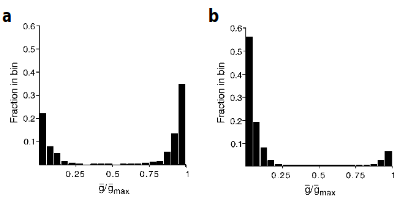
\includegraphics[width=1\textwidth]{CN2}
			\caption{Stationary distribution of synaptic conductances \cite{article}}}
		\end{figure}
	\end{column}
\end{columns}

\note{Integrate and fire: Neuron modeled by its membrane voltage that involves in time with input current}
\end{frame}

\begin{frame}{Stationary distribution II}
	\begin{columns}
		\begin{column}{0.5\textwidth}
			\begin{itemize}
				\item<1-> Regulatory effect on postsynaptic firing rate\\
				
				\item<2-> For all input frequencies: Same ratio of inhibitory and excitatory conductances
				
			\end{itemize}
			
		\end{column}
		\begin{column}{0.5\textwidth}
			\begin{figure}
				
				\centering
				\visible<1->{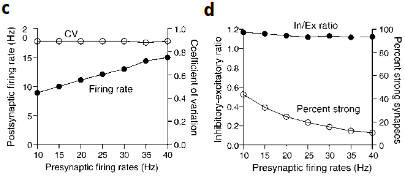
\includegraphics[width=1\textwidth]{CN3}
					\caption{Stationary distribution of synaptic conductances \cite{article}}}
			\end{figure}
		\end{column}
	\end{columns}
\end{frame}
\section{Summary}
\begin{frame}{Summary}
\visible<1->{Advantages:}
\begin{itemize}
	\item<2-> Synapses only adapted based on causal relationships rather than chance 
	\item<3-> Competition arises naturally to maintain equilibrium distribution
\end{itemize}
\visible<4->{Disadvantages:}
\begin{itemize}
	\item<5-> Requires a few assumptions to reach equilibrium distribution like nonlinear spike-generation process
	\item<6-> Postsynaptic firing rate is \textcolor{darkred}{sole} source for synaptic adaptiation! What if excitatory synapses aren't strong enough to begin with?
\end{itemize}
\note{GDML: gradient domain machine learning}
\note{not chemically accurate, since still approximative, but way better than empirical FFs}
\note{Coulomb: electrostatic forces over distances outside curoff radius}
\end{frame}

\begin{frame}{References}
\bibliography{literatur}
\end{frame}
\end{document}